\documentclass[12pt]{article}
\usepackage{enumerate}
\usepackage{notes}

\begin{document}
\title{Oxford A1 - Differential Equations \footnotetext{\url{https://courses.maths.ox.ac.uk/node/5372}}}
\author{Dan Davison}
\maketitle

\section{Sheet 1}

\newpage
\subsection*{}
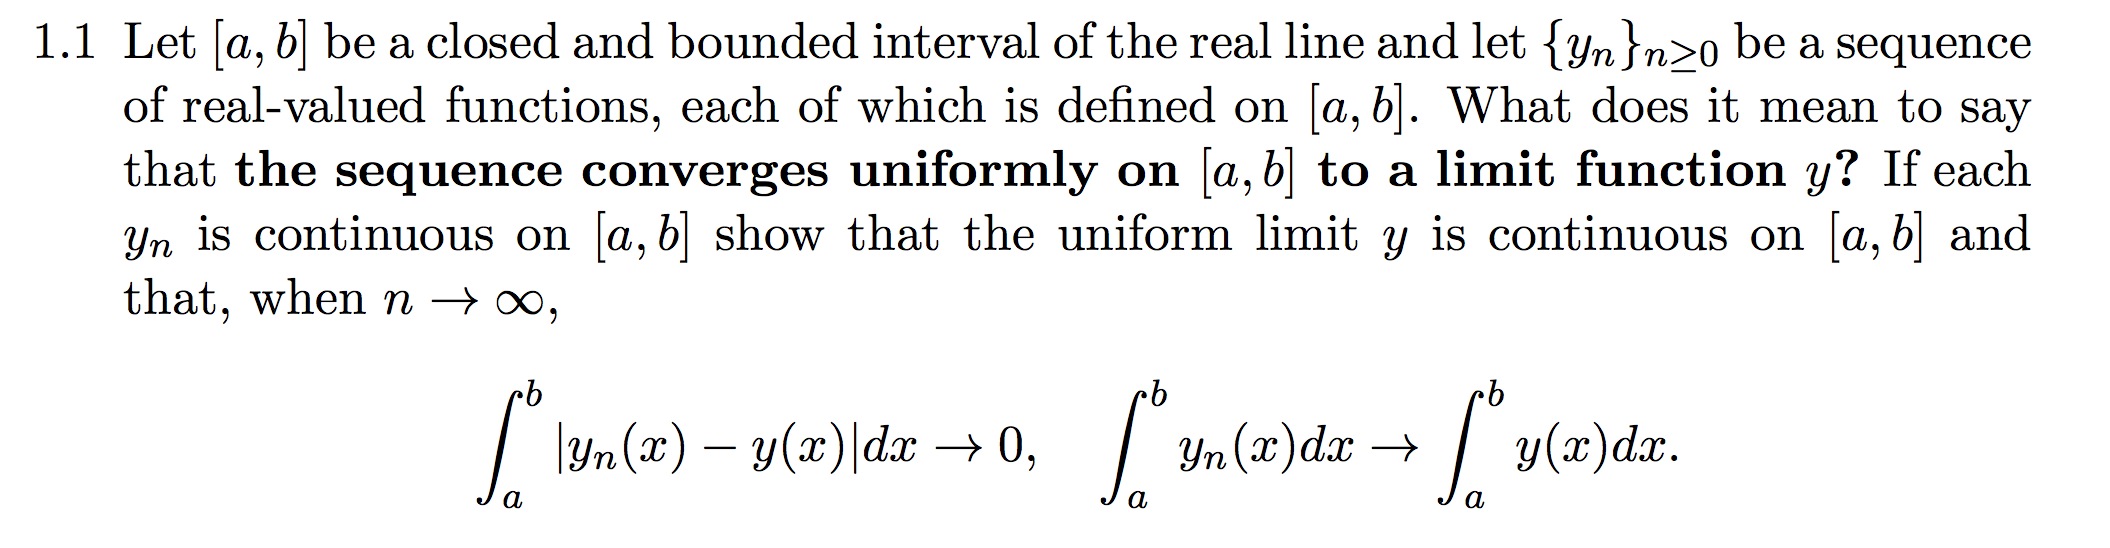
\includegraphics[width=450pt]{img/differential-equations-a1-1-1-a.png}\\
\begin{mdframed}
  \subsubsection*{(a) Definition of uniform convergence}
  The sequence of functions $\{y_n\}_{n\geq 0}$ \textbf{converges uniformly on
    $[a, b]$ to $y$} if and only if for every $\epsilon > 0$ there exists an
  $m \in \N$ such that for every $n > m$, $y_n$ differs from $y$ by no more
  than $\epsilon$ at every point in $[a,b]$.

  \subsubsection*{(b) Show that the limit function is continuous}

  We are told that $\{y_n\}_{n \geq 0}$ converges uniformly to $y$.

  The claim is that if each $y_n$ is continuous on $[a,b]$ then $y$ is
  continuous on $[a,b]$.

  We need to show that for every $\epsilon > 0$, and for every
  $x_0 \in [a, b]$, there exists a $\delta > 0$ such that
  $|x - x_0| < \delta \implies |y(x) - y(x_0)| < \epsilon$.



  We prove this by induction on $n$.

  We are told that $y_0$ is continuous on $[a,b]$.

  Now assume that $y_i$ is continuous on $[a,b]$; we need to show that
  $y_{i+1}$ is continuous on $[a,b]$.

  Fix arbitrary $\epsilon > 0$ and $x_0 \in [a,b]$. Let $m \in \N$ be such that
  for every $n > m$, $y_n(x_0)$ differs from $y(x_0)$ by no more than
  $\epsilon$ at every point of $[a,b]$. We know that $m$ exists, since the
  sequence of functions converge uniformly to $y$.

  Since $y_i$ is continuous on $[a,b]$, there exists a $\delta > 0$ such that
  $|x - x_0| < \delta \implies |y_i(x) - y_i(x_0)| < \epsilon$.

  Therefore

  \subsubsection*{(c) Show that the definite integrals converge}

\end{mdframed}

\newpage
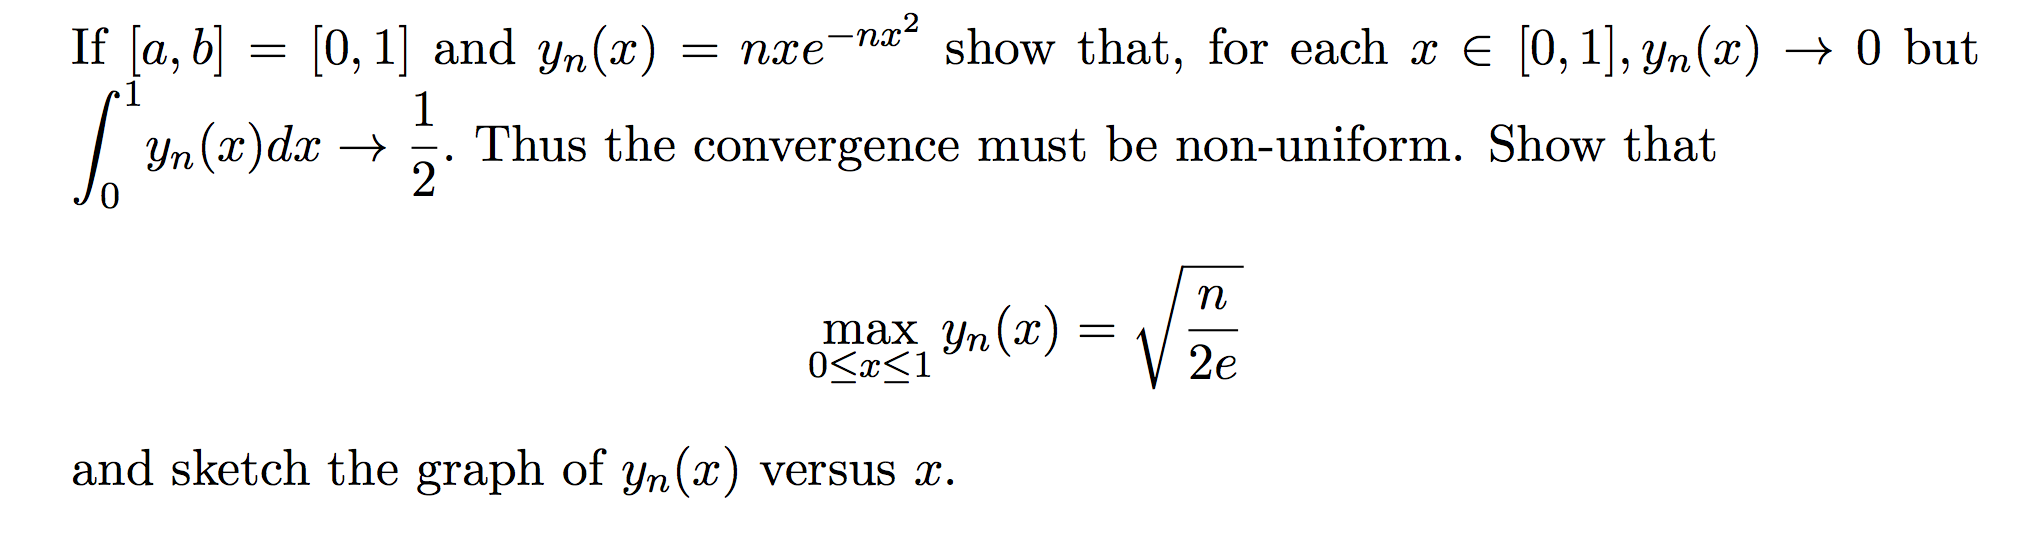
\includegraphics[width=450pt]{img/differential-equations-a1-1-1-b.png}\\
\begin{mdframed}
\end{mdframed}

\end{document}
